% Put the project assessment here

\section{Project Assessment}
    \subsection{User Testing (To Be Expanded on IS295b)}
    The goal here is to ensure that the system works correctly, is easy to use, and meets the needs of its users, especially members of the Ivatan community. The following testing process is planned:\\
    Around 5–10 initial users will be invited to try out the system as test Participants. These may include a mix of students, educators, and community members familiar with Ivatan language and folklore.

    \begin{itemize}
        \item Functional testing: Each feature- dictionary entries, playing audio, submitting folklore stories, will be checked to see if it works properly.
        \item Usability testing: Participants will be asked to complete simple tasks while giving feedback on ease of use, layout, and design.
        \item Bug reporting: Any errors or unexpected behavior will be documented by the proponent or through user feedback forms.
        \item Test Participant can fill out a form such as the one below:
            \begin{figure}[h]
                \centering
                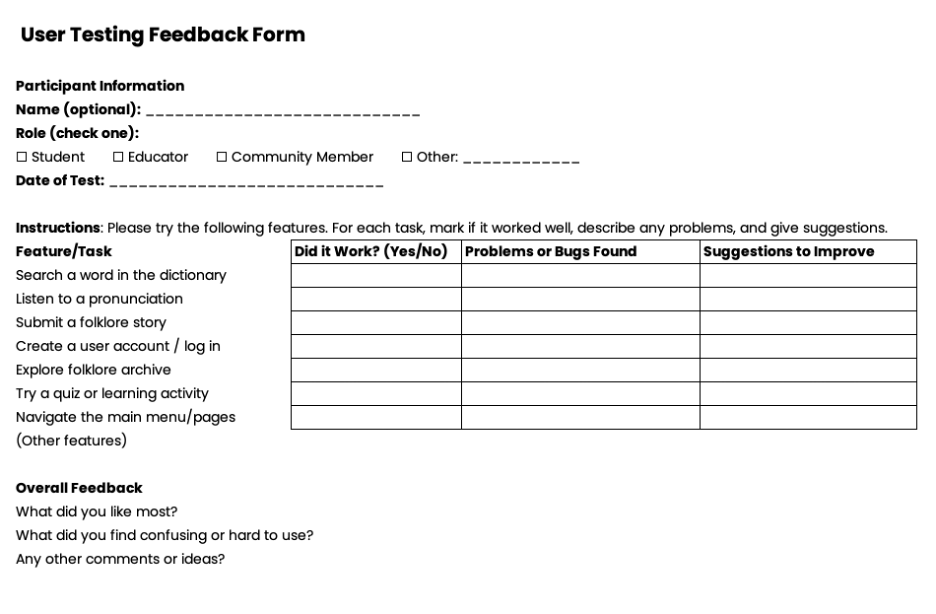
\includegraphics[width=480px]{Texfiles//images/feedbackform.png}
                \caption{User Testing Feedback Form}
            \end{figure}
        \item Bug Fixing and Improvements: After identifying bugs, the proponent will review the code, fix the issues, and re-test the features to ensure they work. 
        \item Regression Testing: After fixing any bugs, the affected features and related parts of the system will be tested again to make sure nothing else broke during the fixes.
    \end{itemize}
\textit{    This section will be completed with actual results and screenshots during IS295B after the final system is built and tested.}



    \subsection{Security Testing (To Be Expanded on IS295b)}
        Security testing will be done after the system is developed to check for common vulnerabilities that could affect user data and content contributions. Planned security considerations include:
        \begin{itemize}
        \item Password Protection: User passwords will be securely stored using hashing .
        \item Input Validation: The system will include input checks to prevent invalid or dangerous data.
        \item Role-Based Access: Different levels of access will be assigned to users like contibutors and reviewers to protect sensitive actions like deleting or approving content.
        \item Secure Hosting: The platform will be hosted using services that offer HTTPS encryption to protect data in transit.
        \item Security Testing Tools: Simple tools available or Django’s built-in security reports will be explored to identify vulnerabilities. Weaknesses found will be noted based on documentation and the system will be re-tested after each fix to make sure it remains secure. 
    \end{itemize}
\textit{    This section will be completed with actual results and screenshots during IS295B after the final system is built and tested.}

